\documentclass[a4paper,12pt]{article}

% Packages
\usepackage[utf8]{inputenc}
\usepackage[T1]{fontenc}
\usepackage[french]{babel}
\usepackage{amsmath,amsfonts,amssymb}
\usepackage{graphicx}
\usepackage{geometry}
\usepackage{fancyhdr}
\usepackage{lastpage}
\usepackage{lipsum} % Pour générer du faux texte. À retirer dans le document final.
\usepackage{natbib}

% Paramètres de la page
\geometry{top=2.5cm, bottom=2.5cm, left=3cm, right=3cm}
\pagestyle{fancy}
\fancyhf{}
\rhead{Caucheteux Maxence}
\lhead{Exercices Statistiques}
\rfoot{Page \thepage/\pageref{LastPage}}
\renewcommand{\headrulewidth}{2pt}
\renewcommand{\footrulewidth}{1pt}
\setlength{\parindent}{0pt}

% Titre du document
\title{Exercices Statistiques}
\author{Maxence Caucheteux}
\date{\today}

% Macros
\newcommand{\E}{\mathbb{E}}
\newcommand{\prob}{\mathbb{P}}
\newcommand{\R}{\mathfrak{R}_0}
\newcommand{\Hun}{H^1(\Omega)}
\newcommand{\Ho}{H^1_0(\Omega)}
\newcommand{\vois}{\mathring{\mathcal{U}}}

\begin{document}

\maketitle

\textbf{Exercice 1.A.6} (Taux de mortalité)

\textbf{Q1/}
On a par calcul direct :
$$\boxed{
\prob(T \in ]t,t+h] \ | \ T>t) =
\left\{
    \begin{array}{ll}
    \frac{F(t+h) - F(t)}{1 - F(t)} & \text{si } F(t) < 1, \\
    0 & \text{sinon}.
    \end{array}
\right.}
$$

\textbf{Q2/}
Comme $p$ est continue, $F$ est $\mathcal{C}^1$ de dérivée $p$ et on a :
$$\boxed{
\mu(t) =
\left\{
    \begin{array}{ll}
    \frac{p(t)}{1 - F(t)} & \text{si } F(t) < 1, \\
    0 & \text{sinon}.
    \end{array}
\right.}
$$


\textbf{Q3/} À la naissance, le taux de mortalité n'est pas nul. En effet, la mortalité infantile explique ce phénomène. Dans les premières années de vie, le taux de mortalité chute car plus un nouveau né grandit, moins il a de chance de décéder prématurément (la mortalité infantile diminue). Vers l'âge de $5$ ans, le taux de mortalité se met à croître, jusqu'à atteindre $0,8$ vers $100$ ans : passées les premières années de vie, plus on vieillit, plus on a de chances de mourir. \\

\textbf{Q4/} Si $T \sim \mathcal{E} (\lambda)$, alors pour tout $t \in \mathbb{R}$, on a $p(t)=\mathbf{1}_{ \{ t>0 \} }\lambda e^{-\lambda t}$. De sorte que :
$$F(t)=\int_{0}^t \lambda e^{-\lambda t} dt = 1-e^{-\lambda t}$$
Bilan : pour $t \geq 0$, $\boxed{\mu(t)=\mathbf{1}_{\{t > 0\} } \lambda}$. \\

\textbf{Q5/ a/} On a $p(t)=F'(t)=(\lambda + \alpha e^{\beta t})e^{-(\lambda t + \frac{\alpha}{\beta}(e^{\beta t} - 1))}$. De sorte que :
$$\boxed{\mu(t)=\lambda + \alpha e^{\beta t}}$$

\textbf{b/} Le phénomène selon lequel un nouveau né a de moins en moins de chances de décéder plus les mois/années après sa naissance n'est pas pris en compte dans ce modèle. En effet, $\mu$ est fonction croissante du temps. \\

\textbf{c/} Si $\alpha > 0$, il est clair que $\frac{\mu(t+1)}{\mu(t)} \sim_{t \infty} e^{\beta}$. En temps long, chaque année le taux de mortalité est multiplié par $\boxed{e^{\beta}}$ par rapport à l'année précédente. Si $\alpha = 0$, $\mu$ est constante égale à $\lambda$ et le facteur recherché est alors $1$. \\

\textbf{d/} Le taux de mortalité est à $30$ ans $\tau_{30}=0,001$ et à $100$ ans $\tau_{100}=0,8$. Ainsi, via l'estimation fondée que la question précédente, on a $\tau_{30}e^{70 \beta} = \tau_{100}$. Donc :
$$\boxed{\beta = \frac{1}{70} \ln \left( \frac{\tau_{100}}{\tau_{30}} \right) \simeq 0,095}$$

\textbf{Q6/} On note $S(t)=\prob (T > t)$ la fonction de survie. On pose $f(t)=\ln S(t) = -(\lambda t + \frac{\alpha}{\beta} (e^{\beta t } -1))$. Ainsi, pour $t_1, t_2$ assez grands, on approxime $\beta \simeq \text{ln} \left( f(t_2)/f(t_1) \right) / (t_2-t_1)$. \\

De plus $f'(t)=-(\lambda+\alpha e^{\beta t})$, $f''(t)=-\alpha \beta e^{\beta t}$. En particulier $f''(0)=-\alpha \beta$, ce qui nous permet d'approximer $\alpha$ en estimant la dérivée seconde de $f$ via les taux de variations. Enfin, en remarquant que $f'(0)=-(\lambda + \alpha)$, on obtient $\lambda$. \\

\begin{figure}[h!]
    \centering
    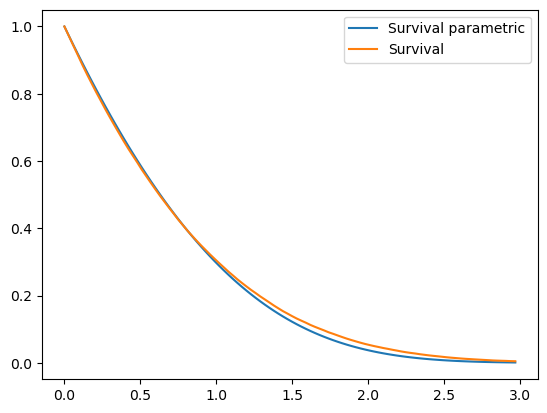
\includegraphics[width=0.8\textwidth]{graphe_survival.png}
    \caption{Graphe de $S$ (bleu : avec paramètres / orange : donné par le csv)}
    \label{fig:graphe_survival}
\end{figure}

On obtient numériquement $\alpha = \simeq 0,668$, $\beta \simeq 0,701$, $\lambda \simeq 0,308$. \\

\textbf{Exercice 1.A.7} (Loi de Cauchy) \\
\textbf{Q1/} Par critère d'intégrabilité de Riemann, on constate que $\boxed{X \notin L^1}$. \\

\textbf{Q2/} Pour $f$ mesurable bornée, on a :
\begin{align*}
\E (f(cX)) &= \int_{\mathbb{R}} f(cx) \frac{a}{\pi} \frac{1}{x^2 + a^2} dx \\
&= \int_{\mathbb{R}} f(u) \frac{a|c|}{\pi} \frac{1}{u^2 + (a|c|)^2} du \ \ \text{cdv} \ u=cx
\end{align*}
Donc $\boxed{X \sim \mathcal{C} (|c|a)}$. \\

\textbf{Q3/} Pour $f$ mesurable bornée, on a :
$$\E \left(f \left( \frac{U}{V} \right) \right) = \frac{1}{2 \pi \sigma \tau} \int_E f(u/v) e^{-u^2/2\sigma^2}e^{-v^2/2 \tau^2} du dv$$
où $E=\{ (u,v) \in \mathbb{R}^d \ | \ u,v \neq 0 \}$.
On effectue alors le changement $(R,S)=(u/v, uv)$. Rigoureusement, on considère le $\mathcal{C}^1$-difféomorphisme suivant :
$$
\varphi : \begin{array}{rcl}
E & \to & F \\
(u,v) & \mapsto & (u/v, uv)
\end{array}
$$
où $F = (\mathbb{R}_{+}^* \times \mathbb{R}_{+}^*) \cup (\mathbb{R}_{-}^* \times \mathbb{R}_{-}^*) \cup (\mathbb{R}_{+}^* \times \mathbb{R}_{-}^*) \cup (\mathbb{R}_{-}^* \times \mathbb{R}_{+}^*)$.

Un calcul montre que $J_{\varphi}(u,v) = 2\frac{u}{v}=2R$. De sorte que :
$$ \int_E f(u/v) e^{-\frac{u^2}{2 \sigma^2}} e^{- \frac{v^2}{2 \tau^2}} du dv = \int_F f(R) e^{- \frac{RS}{2 \sigma^2}} e^{-\frac{S/R}{2 \tau^2}} \frac{1}{2R} dR dS$$

Le domaine $F$ s'écrit comme l'union disjointe de quatre domaines de $\mathbb{R}^2$. Pour commencer, on effectue le calcul sur un de ces quatre domaine, disons $(\mathbb{R}_+^*)^2$. Via Fubini, on a :
\begin{align*}
\int_{(\mathbb{R}_+^*)^2} f(R) e^{- \frac{RS}{2 \sigma^2}} e^{-\frac{S/R}{2 \tau^2}} \frac{1}{2R} \, dR \, dS 
&= \frac{1}{2} \int_0^{+\infty} \frac{f(R)}{R} \left( \int_0^{\infty} e^{-\left(\frac{R}{2\sigma^2} + \frac{1/R}{2\tau^2}\right)S} \, dS \right) \, dR \\
&= \int_{0}^{\infty} f(R) \frac{1}{\frac{R^2}{2\sigma^2} + \frac{1}{2\tau^2}} \, dR
\end{align*}

On remarque via des changements de variables (changements de signe) que le calcul des trois intégrales restantes se ramène au calcul de l'intégrale ci-dessus. D'où l'on tire (après calcul minutieux) : 
$$\E \left(f \left( \frac{U}{V} \right) \right) = \frac{\sigma / \tau}{\pi} \int_{\mathbb{R}} f(R) \frac{dR}{R^2+ \left( \frac{\sigma}{\tau} \right)^2}$$
Conclusion : $\boxed{X \sim \mathcal{C}(| \sigma | / |\tau| )}$. \\

\textbf{Q4/ a/} Pour $x \in \mathbb{R}$, 
\begin{align*}
\Psi_U(x) &= \int_{\mathbb{R}} e^{iux} \frac{a}{2} e^{-a|u|} du \\
&= \frac{a}{2} \left( \int_{0}^{\infty} e^{(ix-a)u} du + \int_{-\infty}^{0} e^{(ix+a)u} du \right) \\
&= \frac{a}{2} \left( \frac{-1}{ix-a} + \frac{1}{ix+a} \right) \\
&\boxed{= \frac{-a^2}{x^2+a^2}}
\end{align*}

\textbf{b/} $\Psi_U$ étant intégrable (continue sur $\mathbb{R}$ et intégrable en $\pm \infty$ via critère de Riemann), on a par Fourier inverse, pour tout $u \in \mathbb{R}$ :
\begin{align*}
p_U(u) &= \frac{1}{2\pi} \int_{\mathbb{R}} e^{-iux} \Psi_U(x) dx \\
&= \frac{-a}{2} \int_{\mathbb{R}} e^{-iux} \frac{a}{\pi} \frac{dx}{x^2+a^2} \\
&= \frac{-a}{2} \Psi_X (-u) 
\end{align*}
D'où, en vertu de l'expression de $p_U(u)$, pour $u \in \mathbb{R}$ : 
$$\boxed{\Psi_X(u)=-e^{-a|u|}}$$

\textbf{c/} Avec $X \sim \mathcal{C}(a)$ et $Y \sim \mathcal{C} (b)$ indépendantes, on a :
\begin{align*}
\Psi_{X+Y}(u) &= \Psi_X(u) \Psi_Y(u) \ \ \text{par indépendance} \\
&= e^{-(a+b)|u|} \ \ \text{par Q4/b/} \\
&= \Phi_Z(u)
\end{align*}
avec $Z \sim \mathcal{C} (a+b)$.
Ainsi : $\boxed{X+Y \sim \mathcal{C} (a+b)}$. \\

\textbf{Q5/a/} Par Q4/, par récurrence immédiate $\sum_{i=1}^n X_i \sim \mathcal{C} (n)$. Par \textbf{Q2/}, $\boxed{\bar{X_n} \sim \mathcal{C}(1)}$. \\

\textbf{b/} On écrit $\bar{X_{2n}} - \bar{X_n}$ comme somme de variables aléatoires indépendantes suivant chacune une loi de Cauchy :
$$\bar{X_{2n}} - \bar{X_n} = \sum_{k=1}^n \frac{-X_k}{2n} + \sum_{k=n+1}^{2n} \frac{X_k}{2n}$$
Or pour $k\in [1,n]$, $\frac{-X_k}{2n} \sim \mathcal{C} (1/2n)$ et pour $k \in [n+1, 2n]$, $\frac{X_k}{2n} \sim \mathcal{C} (1/2n)$ via Q2/. Ainsi via Q4/, on a $\boxed{\bar{X_{2n}} - \bar{X_n} \sim \mathcal{C} (1)}$. \\

\textbf{c/} Si par l'absurde $(\bar{X_n})$ convergeait en probabilité, alors $(\bar{X_{2n}} - \bar{X_n})$ convergerait en probabilité vers $0$ et donc a fortiori en loi vers $0$. Cela contredit la question précédente. Ainsi, $(\bar{X_n})$ ne converge pas en probabilité. \\

\textbf{Exercice 1.A.8} (Convergence plus forte dans le TCL)

\textbf{Q1/} On a $Z_n'=\frac{1}{\sqrt{n}} \sum_{i=1}^n Y_i$ en loi et donc via théorème central limite, $Z_n' \overset{\text{loi}}{\underset{n \to \infty}{\longrightarrow}} \mathcal{N} (0, \sigma^2)$. \\

\textbf{Q2/} Si $Z_n \overset{\mathbb{P}}{\underset{n \to \infty}{\longrightarrow}} Z$, comme $Z_n' = \sqrt{2} Z_{2n} - Z_n$, on en déduit que $Z_n' \overset{\mathbb{P}}{\underset{n \to \infty}{\longrightarrow}} (\sqrt{2}-1)Z \sim \mathcal{N} (0, (\sqrt{2}-1)^2) \sigma^2)$ et donc a fortiori converge en loi vers $\mathcal{N} (0, (\sqrt{2}-1)^2) \sigma^2)$. Mais par la question précédente, $(Z_n')$ converge en loi vers $\mathcal{N}(0, \sigma^2)$. C'est absurde. \\

\textbf{Q3/} $(Z_n)$ ne converge pas en probabilité.

\end{document}